\documentclass[11pt]{article}
\usepackage[a4paper,margin=2.2cm]{geometry}
\usepackage{graphicx}
\usepackage{ctex}
\usepackage{hyperref}
\usepackage{listings}
\usepackage{xcolor}
\hypersetup{colorlinks=true,linkcolor=blue,urlcolor=blue}
\setlength{\parindent}{0pt}
\setlength{\parskip}{6pt}

\title{\bfseries Agent \& MAS Course Assignment\\[2mm]
\large Running, Improving, and Comparing a Multi-Agent Research System\\[1mm]
\normalsize Topic: \textit{LLM-assisted PLC code generation and industrial automation programming}}
\author{mianma05}
\date{October 18, 2026}

\begin{document}
\maketitle

\begin{abstract}
This report documents two tasks. In Task~1 the repository
\texttt{catDforD/LLM\_MAS\_AutoGen} (a three/four-agent research assistant built on
Microsoft AutoGen) was cloned, run locally, and its execution logs were interpreted. In Task~2 the
system was extended with a PLC code-generation and deterministic verification loop, run on the same
topic, and compared with the original. All code, screenshots, and logs are included in the
repository.
\end{abstract}

\section{Task 1 --- Running the Original MAS}

\subsection{Overview}
The original MAS converts a research topic into a short cited report. The \texttt{basic.py}
version uses a fixed pipeline \texttt{PlannerAgent} $\rightarrow$ \texttt{SearchAgent}
$\rightarrow$ \texttt{WriterAgent} on a \texttt{RoundRobinGroupChat}. The \texttt{advanced.py}
version adds a \texttt{ReviewerAgent} and a one-revision loop on a \texttt{SelectorGroupChat} with a
deterministic \texttt{choose\_next} router. The single real tool, \texttt{search\_literature},
queries a bundled course source library and the Crossref API.

\subsection{Run results}
Both versions were run with the PLC topic using the \texttt{deepseek-chat} model. The basic run
produced a five-section report with citations \texttt{[S1]}--\texttt{[S12]}; the advanced run
triggered a review--revision cycle in which the reviewer found citation problems and the writer
revised the report. Figure~\ref{fig:basic} and Figure~\ref{fig:advanced} show the run output.

\begin{figure}[!htbp]
\centering
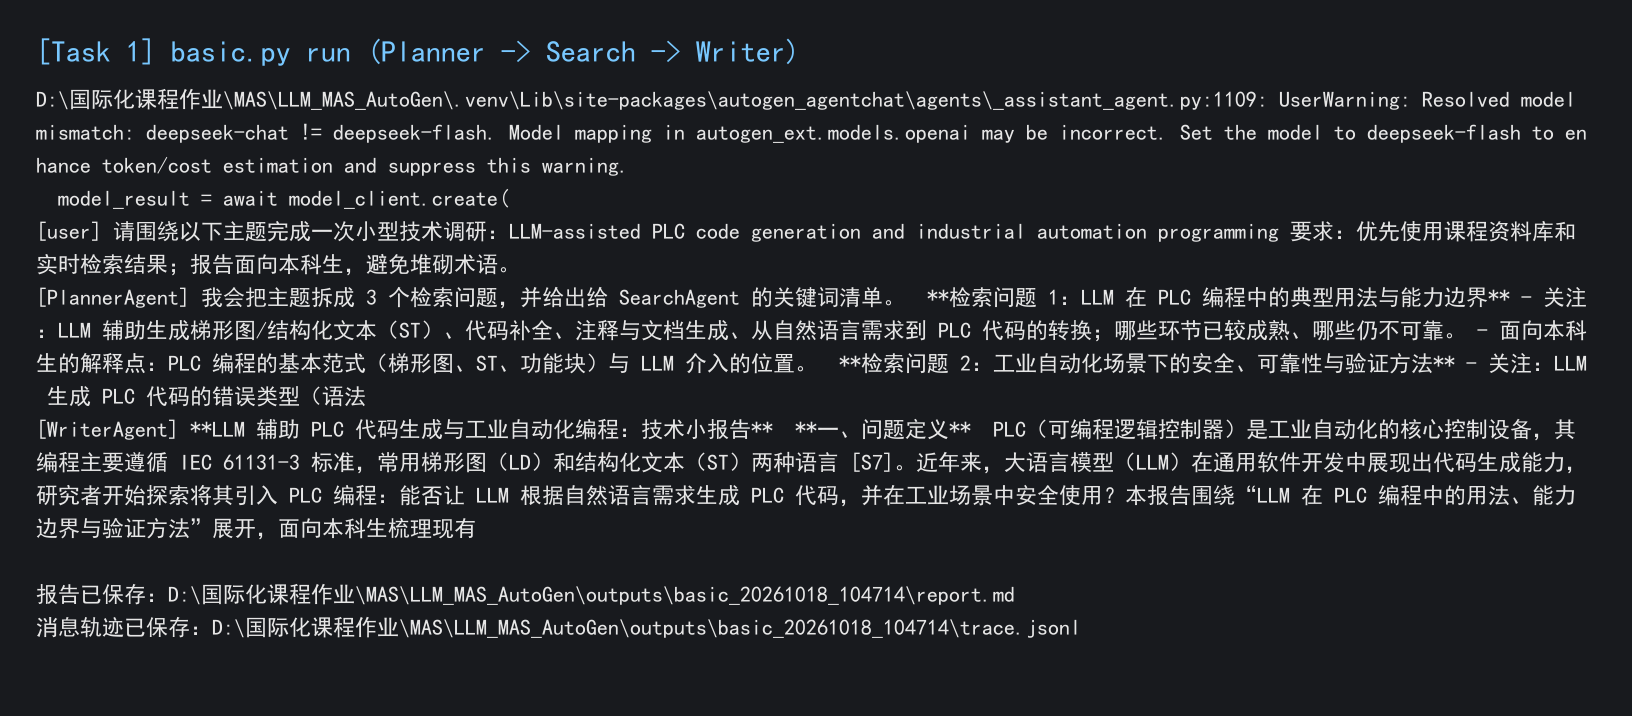
\includegraphics[width=0.9\textwidth,height=0.82\textheight,keepaspectratio]{../screenshots/01_basic_run_console.png}
\caption{Task 1 --- \texttt{basic.py} run (Planner $\rightarrow$ Search $\rightarrow$ Writer).}
\label{fig:basic}
\end{figure}

\begin{figure}[!htbp]
\centering
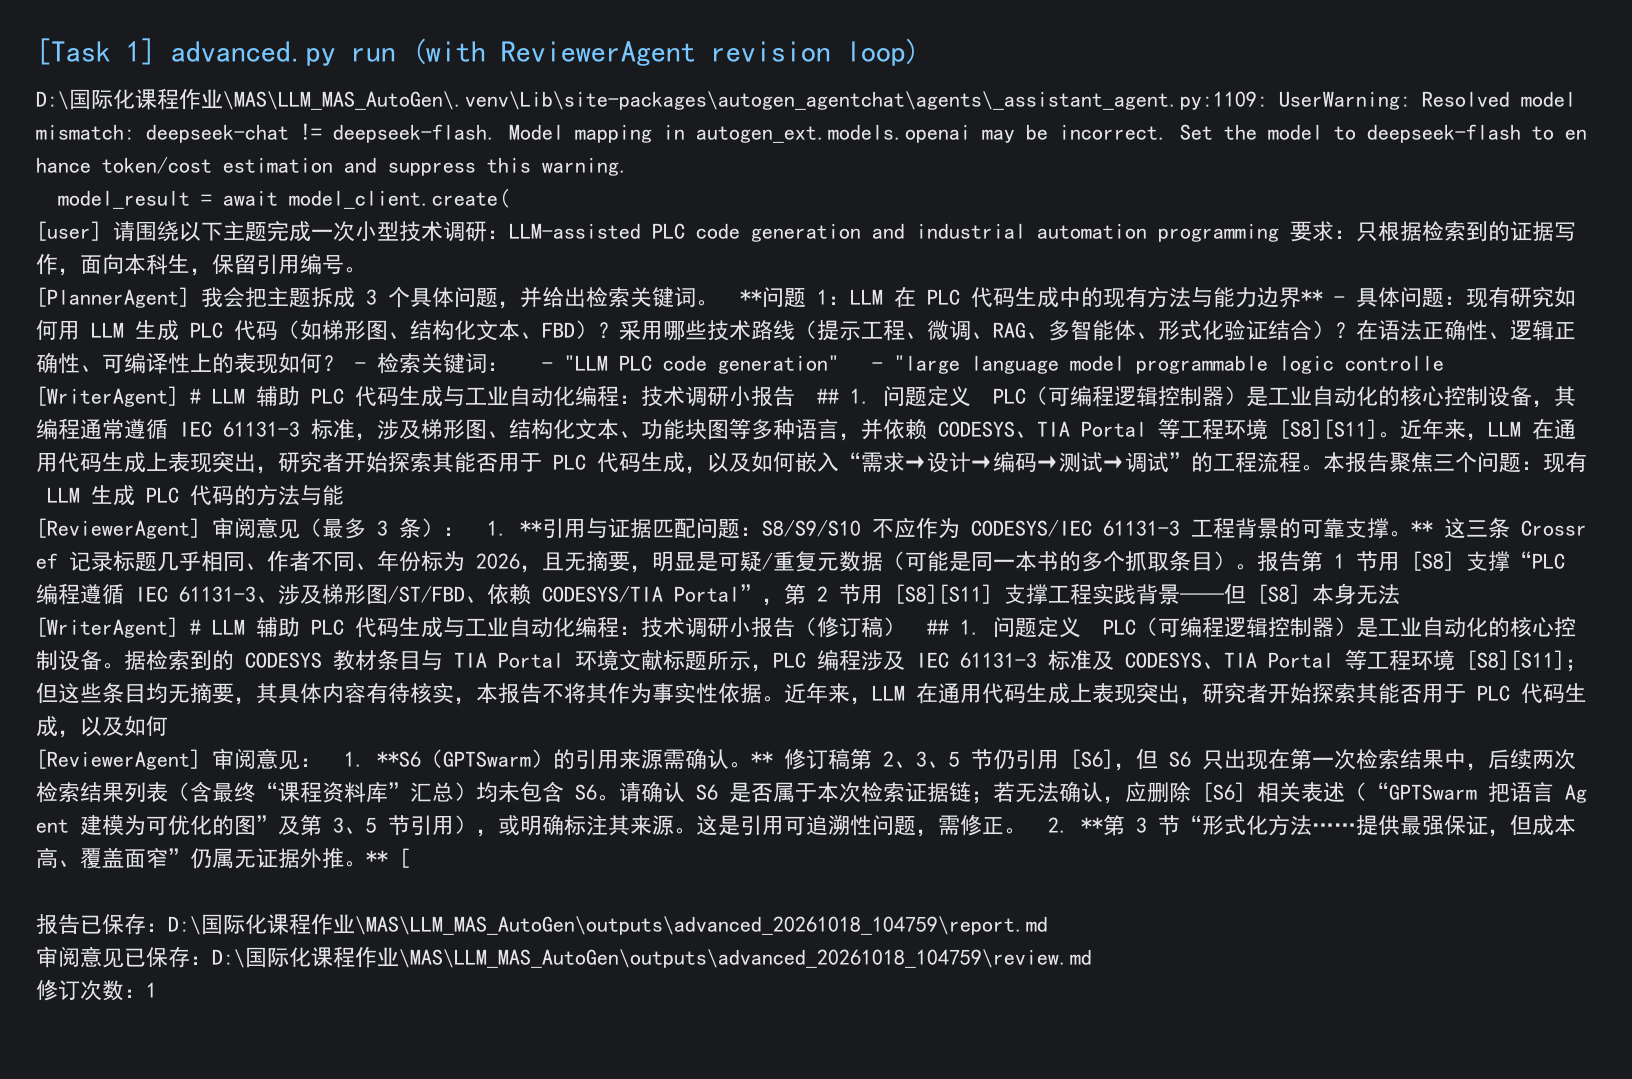
\includegraphics[width=0.9\textwidth,height=0.82\textheight,keepaspectratio]{../screenshots/02_advanced_run_console.png}
\caption{Task 1 --- \texttt{advanced.py} run with the ReviewerAgent revision loop.}
\label{fig:advanced}
\end{figure}

\subsection{Execution-log interpretation}
The trace (\texttt{trace.jsonl}) records every event. Three observations matter:

\begin{enumerate}
\item \textbf{Real tool calls.} \texttt{SearchAgent} issued three \texttt{search\_literature} calls
with different query strings. Each returned an evidence list with \texttt{[S\#]} numbers, linking
the tool result to the later report.
\item \textbf{Agent-to-agent message passing.} The planner's keywords flow into the searcher's tool
calls, whose results are forwarded as \texttt{ToolCallSummaryMessage}s to the writer, which cites
them.
\item \textbf{Termination and evidence traceability.} The basic run stops on the
\texttt{BASIC\_REPORT\_DONE} sentinel; the advanced run stops on \texttt{REVIEW\_APPROVED}/
\texttt{REVISION\_REQUIRED} with a one-revision cap. The \texttt{evidence\_registry.json} maps every
cited \texttt{[S\#]} back to a real source, and \texttt{audit\_citations} verifies it.
\end{enumerate}

Figure~\ref{fig:review} shows the reviewer's feedback and the deterministic citation audit.

\begin{figure}[!htbp]
\centering
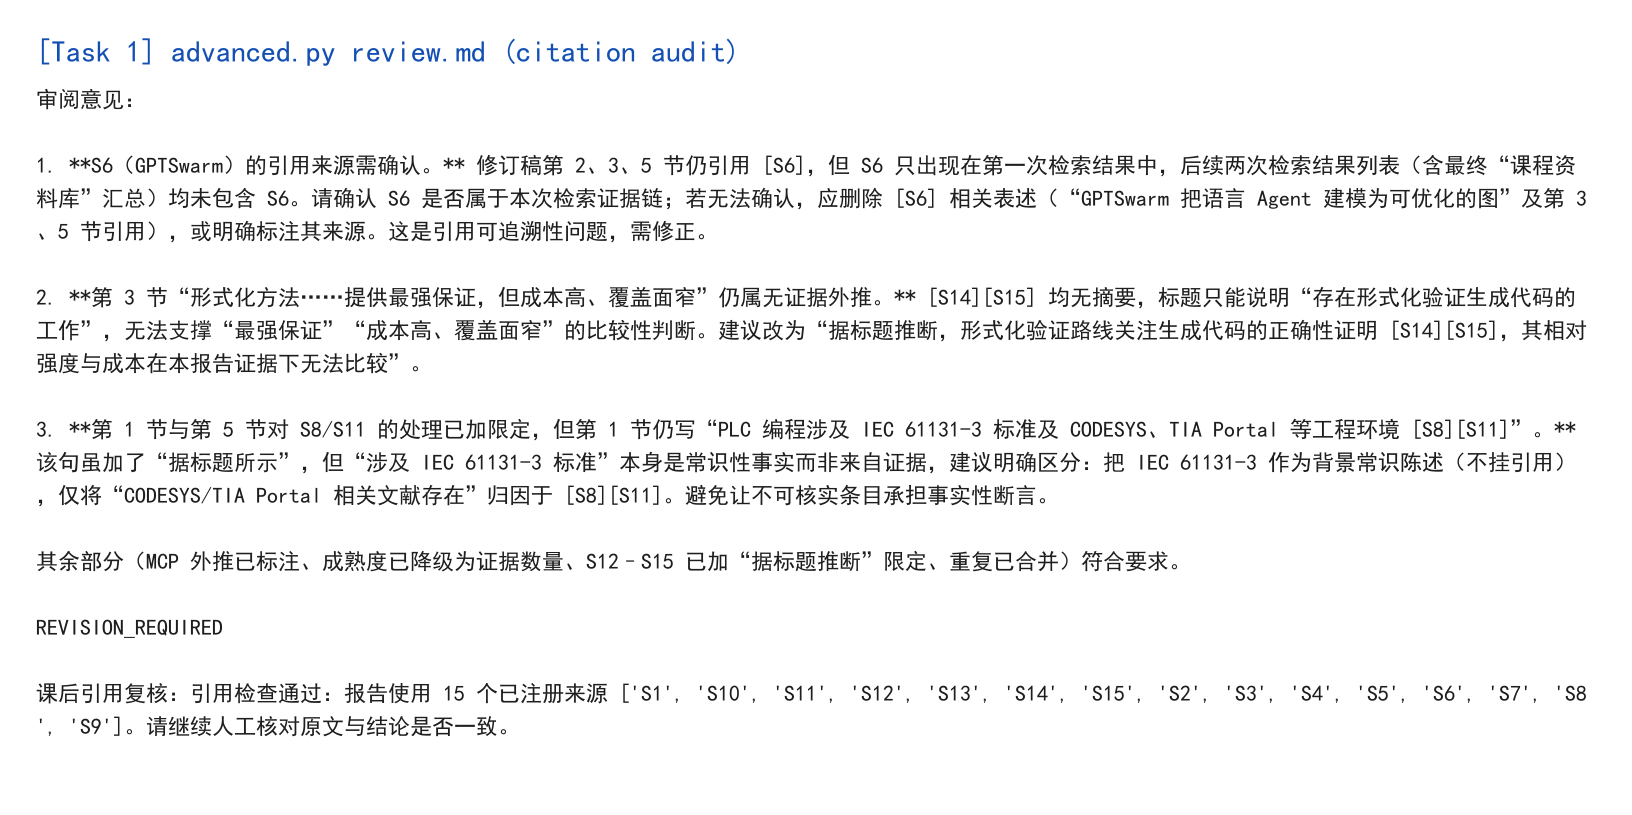
\includegraphics[width=0.9\textwidth,height=0.82\textheight,keepaspectratio]{../screenshots/06_advanced_review.png}
\caption{Task 1 --- \texttt{advanced.py} \texttt{review.md}: reviewer feedback and citation audit.}
\label{fig:review}
\end{figure}

\section{Task 2 --- Improvement: PLC Code Generation \& Verification}

\subsection{Improvement idea}
The original system only \emph{describes} how an LLM-based MAS can generate PLC code. The
improvement makes it \emph{actually generate and verify} PLC code: after the research stage, a new
code stage runs \texttt{CodeGeneratorAgent} $\rightarrow$ \texttt{CodeVerifierAgent}, where the
verifier calls a new deterministic tool \texttt{check\_st\_code} and the result drives a
generate--verify--revise loop.

\subsection{New components}
\begin{itemize}
\item \textbf{CodeGeneratorAgent} --- generates a demo IEC 61131-3 Structured Text (ST) program
(motor start/stop with an emergency-stop interlock and a \texttt{TON} timer).
\item \textbf{CodeVerifierAgent} --- calls \texttt{check\_st\_code} and reports the verdict
(\texttt{reflect\_on\_tool\_use=False}, like the original searcher, for determinism).
\item \textbf{check\_st\_code} (in \texttt{plc\_tools.py}) --- a real, deterministic tool: it strips
comments and checks keyword pairing (\texttt{IF/END\_IF}, \texttt{PROGRAM/END\_PROGRAM}, \dots),
bracket balance, and the misuse of \texttt{=} where ST requires \texttt{:=}. It returns
\texttt{PASS}/\texttt{FAIL}.
\item \textbf{Deterministic routing} --- the code-stage router inspects the tool result directly:
\texttt{FAIL} (and revision budget left) $\rightarrow$ back to the generator; \texttt{PASS}
$\rightarrow$ stop.
\end{itemize}

This satisfies the Task~2 requirements: new roles and architecture, and at least one real tool call
(\texttt{check\_st\_code}) whose result is used later to drive the revision decision.

\subsection{Run results}
The improved MAS was run on the same topic. Figure~\ref{fig:improved} shows the two-stage run.
The generated code passed verification on the first attempt
(\texttt{code\_verification\_pass = true}).

\begin{figure}[!htbp]
\centering
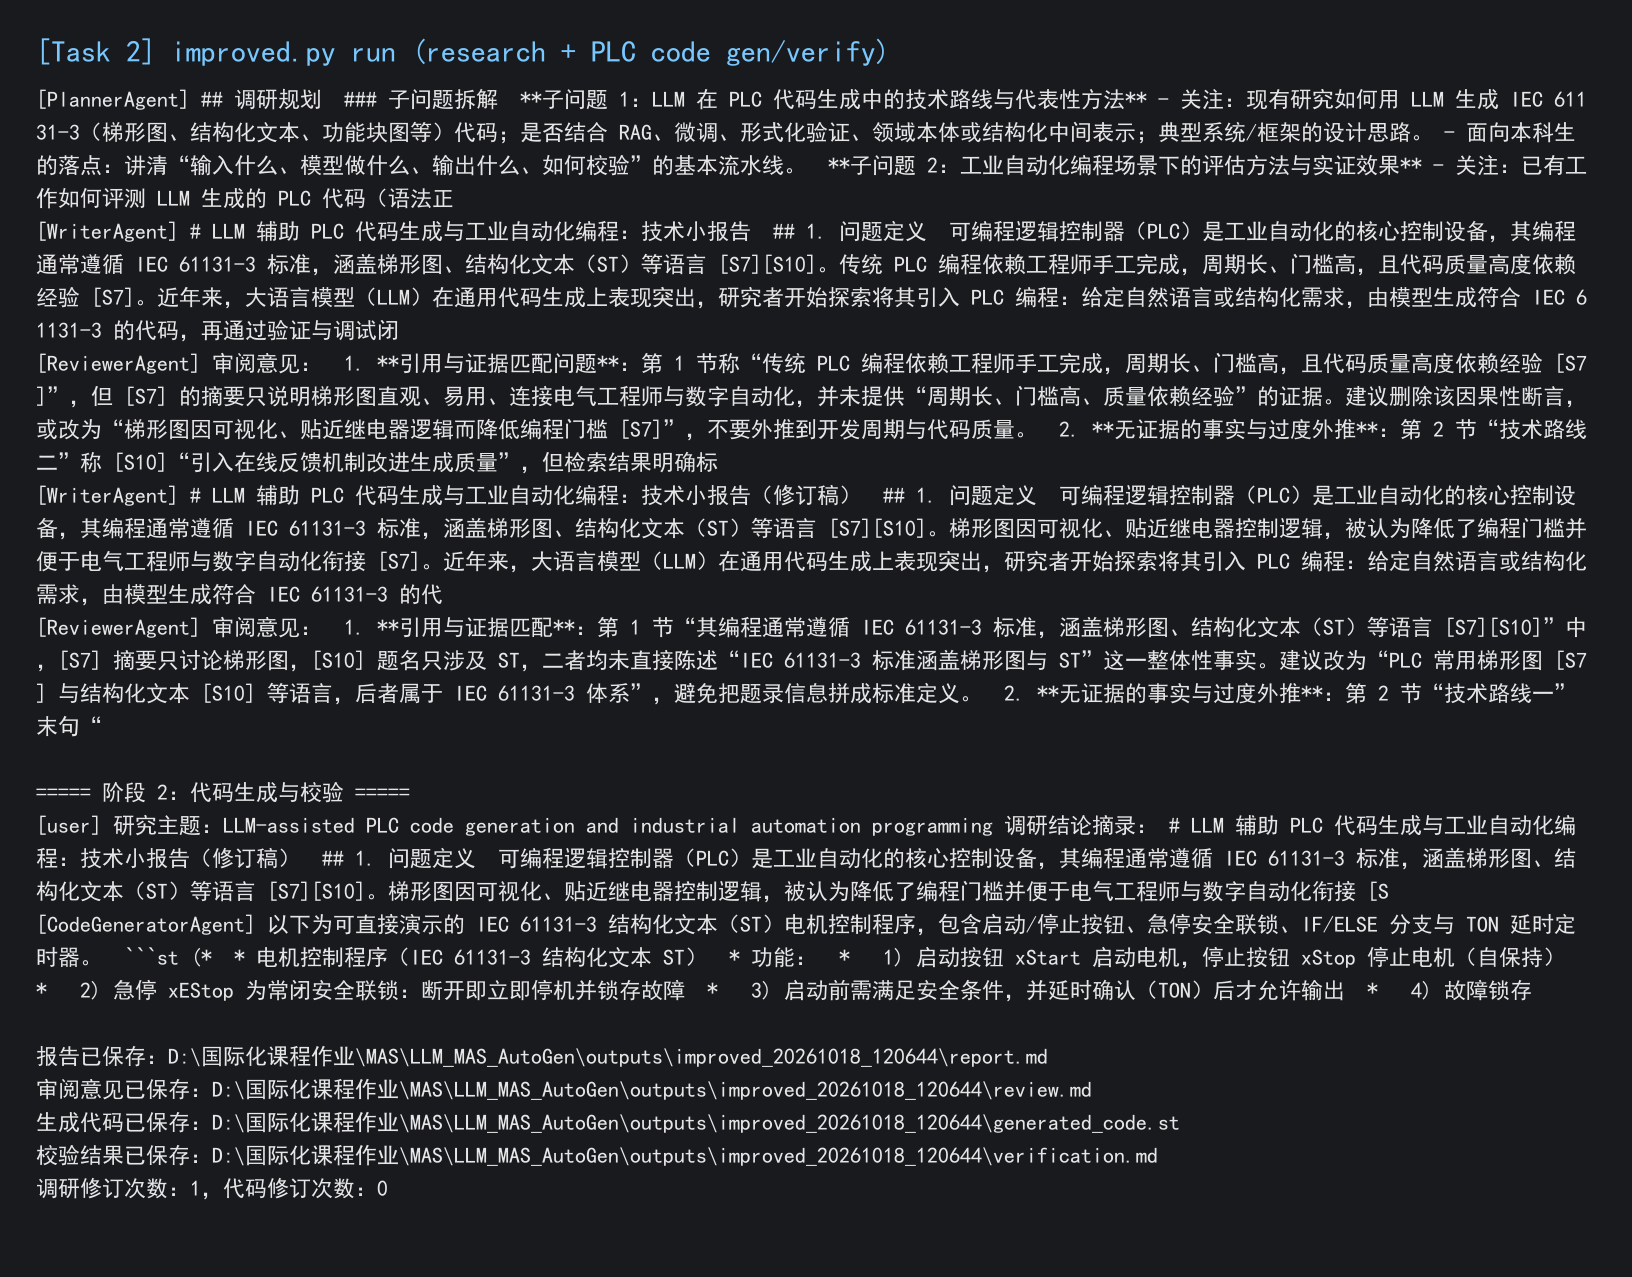
\includegraphics[width=0.9\textwidth,height=0.82\textheight,keepaspectratio]{../screenshots/03_improved_run_console.png}
\caption{Task 2 --- \texttt{improved.py} run (research stage + code stage).}
\label{fig:improved}
\end{figure}

\begin{figure}[!htbp]
\centering
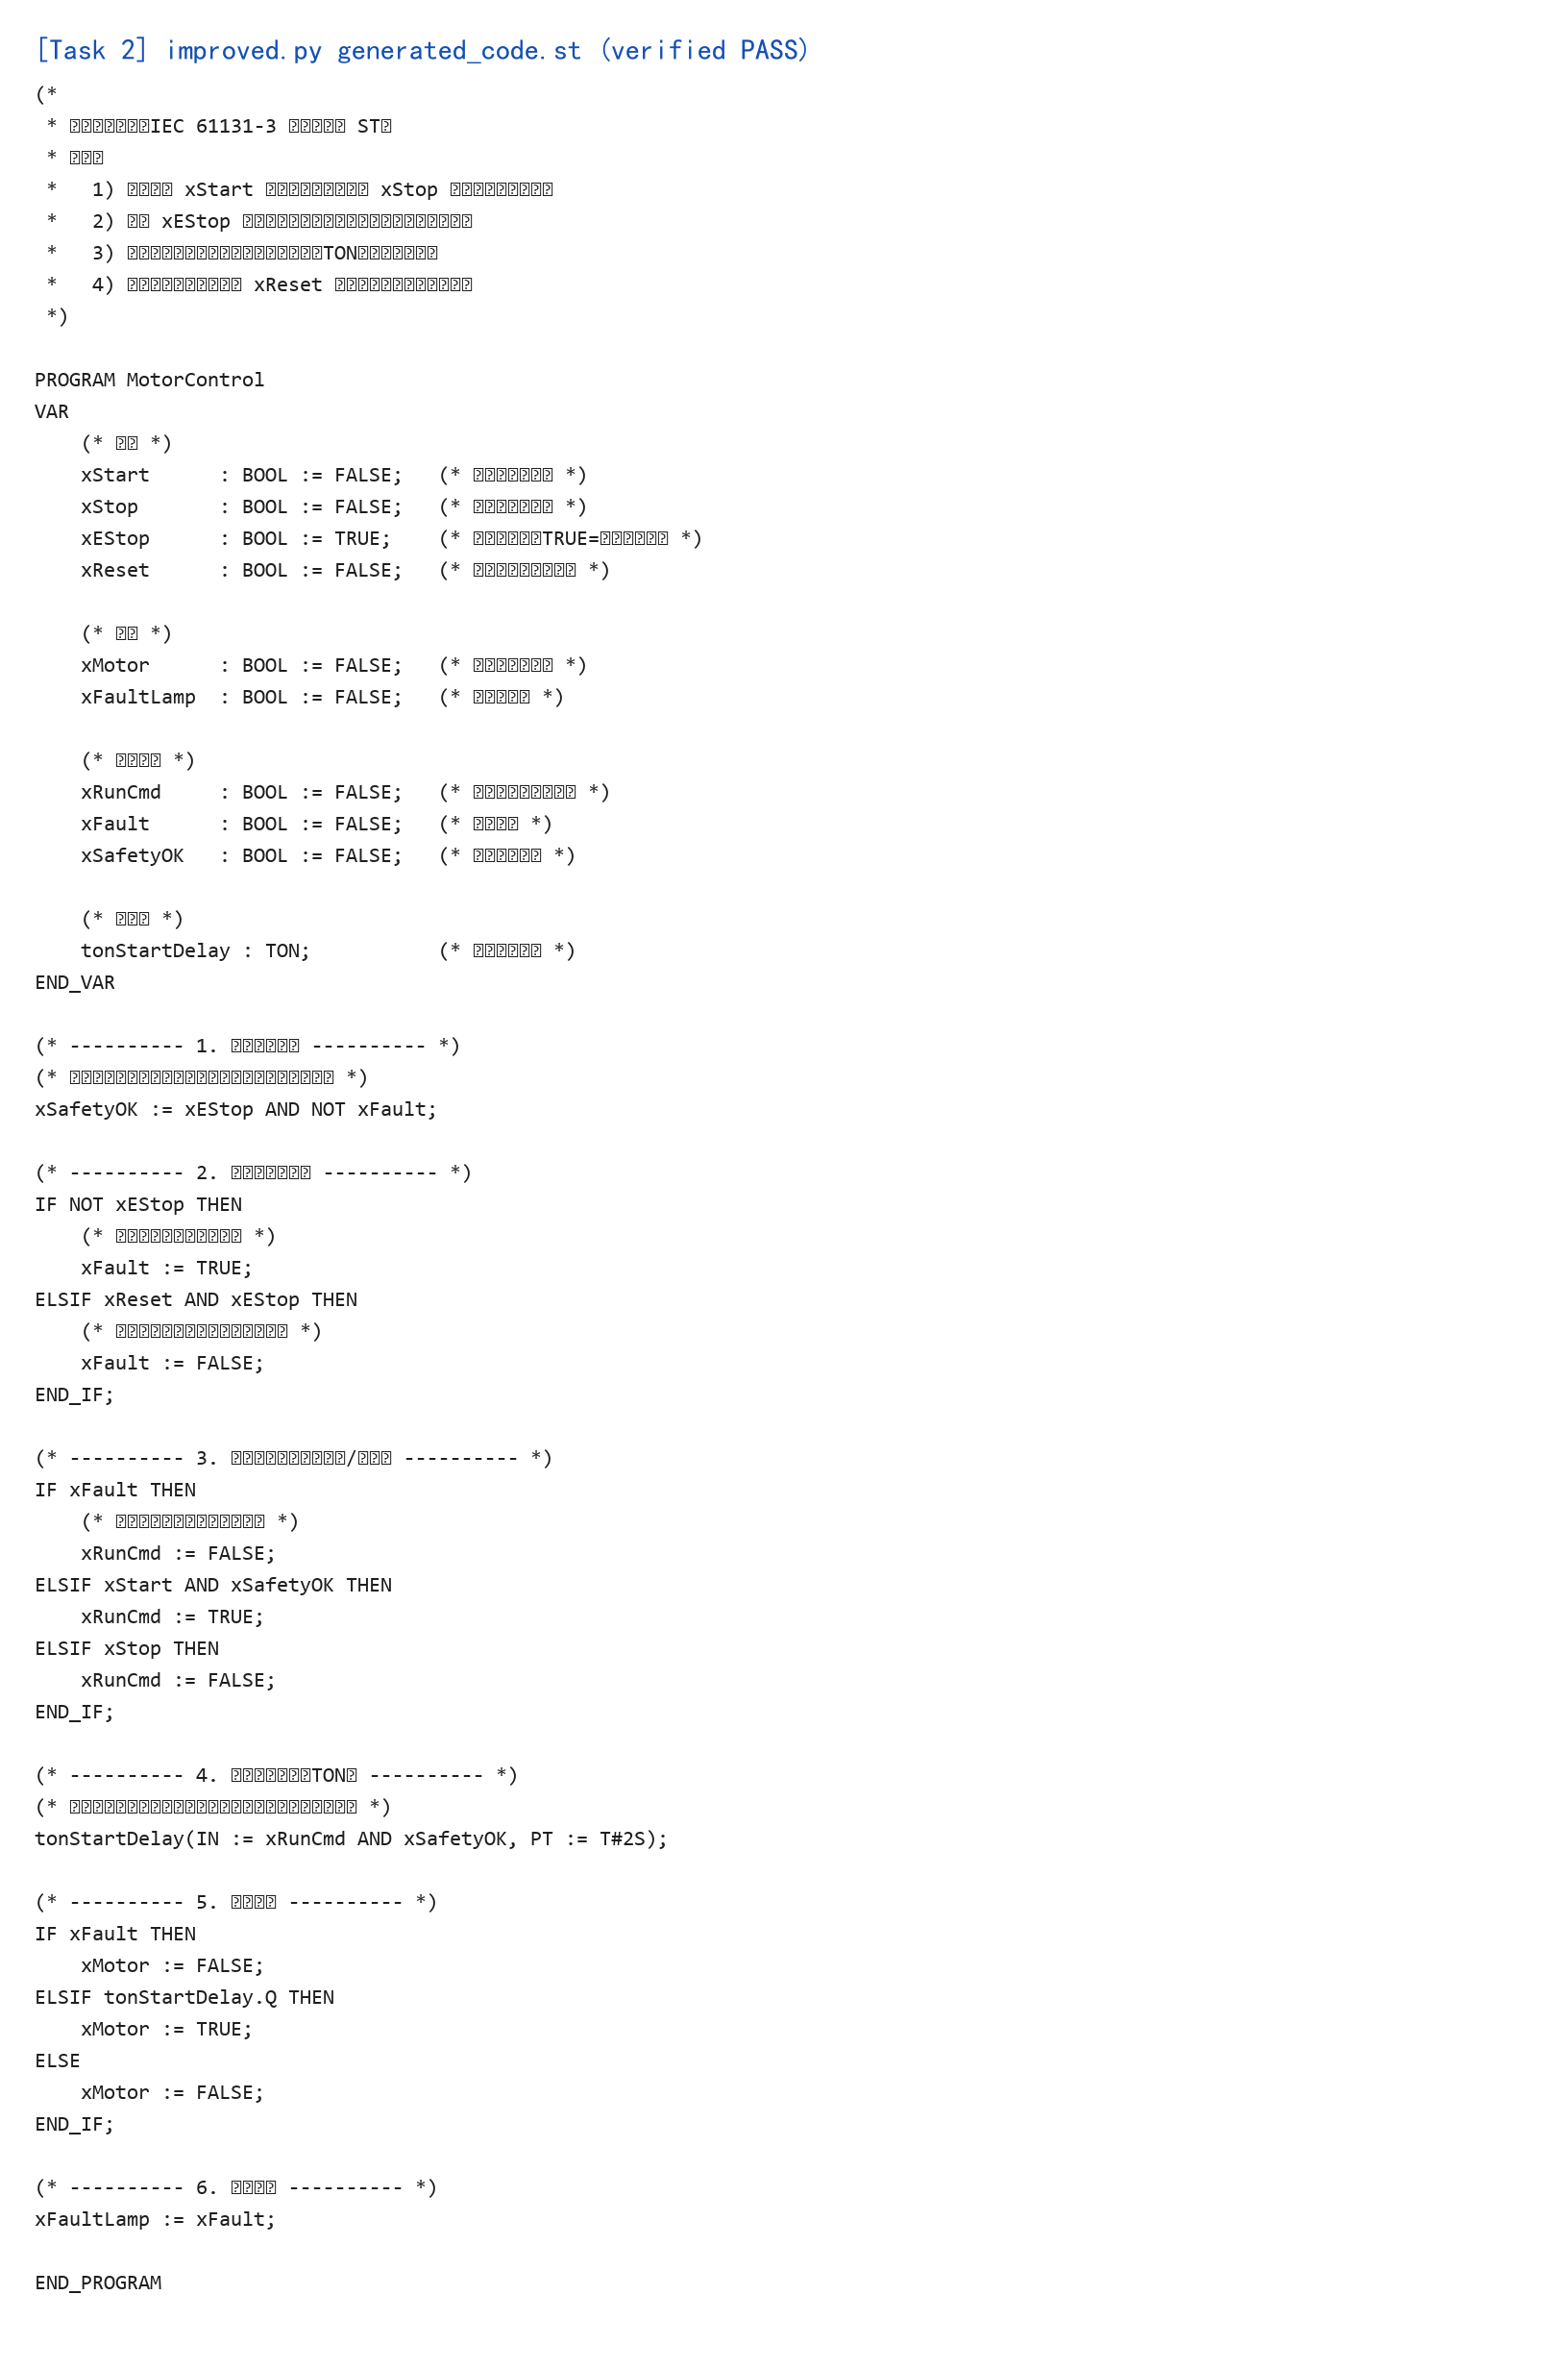
\includegraphics[width=0.9\textwidth,height=0.82\textheight,keepaspectratio]{../screenshots/08_improved_generated_code.png}
\caption{Task 2 --- the verified IEC 61131-3 ST program (\texttt{generated\_code.st}).}
\label{fig:code}
\end{figure}

\begin{figure}[!htbp]
\centering
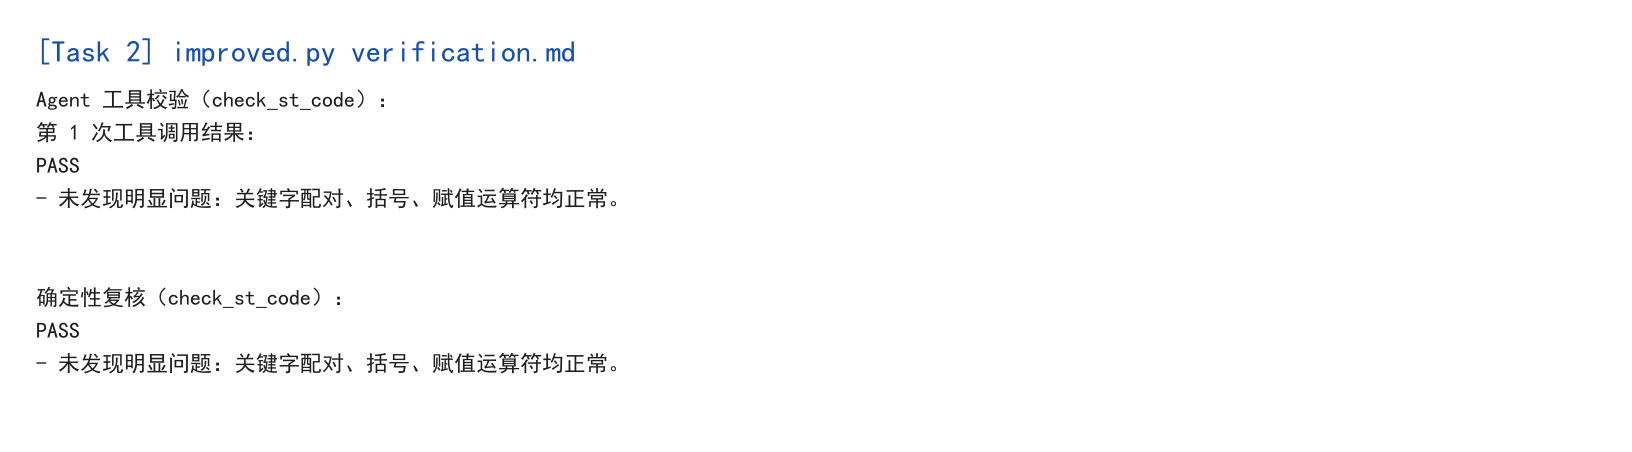
\includegraphics[width=0.9\textwidth,height=0.82\textheight,keepaspectratio]{../screenshots/09_improved_verification.png}
\caption{Task 2 --- \texttt{verification.md}: the \texttt{check\_st\_code} result and deterministic
re-check, both \texttt{PASS}.}
\label{fig:verify}
\end{figure}

\section{Comparison of the Original and Improved MAS}

\begin{center}
\begin{tabular}{p{4.3cm}|p{5.2cm}|p{5.4cm}}
\hline
\textbf{Dimension} & \textbf{Original (\texttt{advanced.py})} & \textbf{Improved (\texttt{improved.py})} \\
\hline
Roles & Planner, Search, Writer, Reviewer & + CodeGenerator, CodeVerifier \\
Output & cited research report & research report + verified ST code \\
Tools & \texttt{search\_literature}, \texttt{audit\_citations} & + \texttt{check\_st\_code} \\
Workflow & one research revision loop & research loop + code generate--verify loop \\
Reliability & citation audit, max turns & + deterministic code verification \\
On-topic value & describes PLC-code MAS & also produces \& checks PLC code \\
\hline
\end{tabular}
\end{center}

The improvement trades a small amount of extra runtime for a much more concrete demonstration: the
MAS now produces and independently verifies domain code instead of only describing it. The
verification is deterministic, so the system does not rely on the LLM to judge its own output --- a
reliability property that is especially important for industrial-control code.

\section{Conclusion}
Both tasks were completed. The original MAS was run and its logs interpreted (Task~1); a PLC
code-generation and verification loop was added, run on the same topic, and compared with the
original (Task~2). The repository contains the full code (with \texttt{README.md}), the two
research reports under \texttt{reports/}, and run screenshots under \texttt{screenshots/}.

\end{document}
